\documentclass[11pt]{article}
% -----------------------------------------------------------------------------
% Dedicated standalone LaTeX document for Reviewer 3, Comment 2 (R3.2):
% Sensitivity analysis to the hyperparameter \gamma and validation-set selection.
%
% Created separately so as NOT to touch response_letter_CPENG-8674.tex while it
% is being edited. Uses the exact preamble, macros, and figure paths
% (./figures_final/) of response_letter_CPENG-8674.tex for direct copy-pasting.
% -----------------------------------------------------------------------------
\usepackage[a4paper,margin=2.5cm]{geometry}
\usepackage{amsmath,amssymb,bm}
\usepackage{graphicx}
\usepackage{booktabs,multirow,array,longtable,tabularx}
\usepackage{xcolor}
\usepackage{caption,subcaption}
\usepackage{float}
\usepackage{enumitem}
\usepackage{titlesec}
\usepackage[colorlinks=true,linkcolor=blue!50!black,citecolor=blue!50!black,urlcolor=magenta]{hyperref}

\definecolor{resp}{RGB}{25,70,170}
\definecolor{note}{RGB}{205,95,0}
\linespread{1.15}
\setlength{\parindent}{0pt}
\setlength{\parskip}{4pt}
\captionsetup{font=small,labelfont=bf,labelsep=colon}
\renewcommand{\thetable}{R\arabic{table}}
\renewcommand{\thefigure}{R\arabic{figure}}
\renewcommand{\theequation}{R\arabic{equation}}
\titleformat{\section}{\normalfont\large\bfseries}{}{0pt}{}
\titleformat{\subsection}{\normalfont\bfseries}{}{0pt}{}
\setlist{itemsep=1pt,topsep=2pt}

% --- Comment / response / action blocks (identical to response_letter_CPENG-8674.tex) ---
\newenvironment{rcomment}[1]{\par\bigskip\noindent\textbf{Comment\ifx&#1&\else\ #1\fi:}\ \itshape}{\par}
\newenvironment{response}{\par\smallskip\noindent\color{resp}\textbf{Response:}\ }{\par}
\newenvironment{action}{\par\smallskip\noindent\color{resp}\textbf{Action:}\ }{\par}
\newcommand{\authornote}[1]{\textcolor{note}{\textsf{[Authors: #1]}}}
\newcommand{\tbd}[1]{\textcolor{note}{\textsf{[#1]}}}
\newcommand{\lines}[1]{\tbd{lines #1}}

\newcommand{\m}{\mathbf{m}}
\newcommand{\z}{\mathbf{z}}
\newcommand{\f}{\mathbf{f}}

\begin{document}

\begin{center}
{\Large\bfseries Dedicated Draft for Reviewer \#3, Comment 2 (R3.2)}\\[6pt]
\textbf{Sensitivity Analysis to the Hyperparameter $\gamma$ and Validation-Based Model Selection}\\[4pt]
\textbf{MANUSCRIPT ID:} CPENG-8674 \quad|\quad \textbf{Date:} \today
\end{center}

% =============================================================================
\section*{Response to Reviewer \#3, Comment 2 (ready to paste into the response letter)}
% =============================================================================

\begin{rcomment}{2}
In the ``Sensitivity to $\gamma$ hyperparameter and model selection'' section, the hyperparameter $\gamma$, which
balances the data likelihood and the prior regularization, is calibrated based on the performance of the model on the
test dataset. This approach compromises the independence of the test set and results in overly optimistic performance
estimates. The optimal value of $\gamma$ must be selected using only the validation dataset. The authors need to
correct this methodological flaw and subsequently report the unbiased performance metrics on the completely unseen test
set.
\end{rcomment}

\begin{response}
We agree with the reviewer, and we have corrected this methodological issue in the revised manuscript. Both the
analysis of $\gamma$ and the selection of the trained model weights are now performed exclusively on the validation
dataset (2,400 observations), so that the test dataset (1,200 observations) remains completely unseen until the final
evaluation.

With respect to the original submission, we have reformulated the data-misfit term of the loss function by calibrating
it with respect to the measurement and modeling error variances (dividing each frequency and mode-shape discrepancy by
its error variance $2\sigma^2$):
\begin{equation}
\mathrm{NLL}(\z;\m)=\tfrac12\,\mathbf{d}^{\top}\bm{\Sigma}_f^{-1}\mathbf{d}
+\sum_{j=1}^{n_m}\frac{1-\mathrm{MAC}_j(\bm{\Phi},\hat{\bm{\Phi}}(\z))}{2\,s_{v,j}^2},\qquad
\mathbf{d}=\log\f-\mathbf{b}-\log\hat{\f}(\z).
\label{eq:nll}
\end{equation}
In the original formulation, the frequency and MAC errors were multiplied by fixed heuristic weights, so the relative
magnitude of the reconstruction term and the differential entropy $\mathcal{H}[q(\z|\m)]$ depended on the unscaled error
units and on the dimensionality of the observations and latent space, requiring $\gamma$ to be tuned empirically. By
rescaling the residuals with the error variances $2\sigma^2$ in Eq.~\eqref{eq:nll}, the data term becomes the true
Gaussian negative log-likelihood $-\log p(\m|\z)$ (in nats), on the exact same scale and units as the differential
entropy of the $D$-dimensional variational posterior. Under the uniform prior on $[0.45,1]^7$, the training loss
\begin{equation}
\mathcal{L}(\bm\theta)=\frac1N\sum_{i=1}^N\Big(\mathbb{E}_{q}\big[\mathrm{NLL}(\z;\m_i)\big]
-\gamma^2\,\mathcal{H}\big[q_{\bm\zeta_{\bm\theta}}(\z|\m_i)\big]\Big)
\label{eq:loss}
\end{equation}
recovers the exact negative Evidence Lower Bound ($-\mathrm{ELBO}$, up to an additive constant) for $\gamma=1$. Varying
$\gamma$ in Eq.~\eqref{eq:loss} is equivalent to dividing $\mathrm{NLL}(\z;\m)$ by $\gamma^2$, i.e., rescaling the
effective error standard deviations $\sigma$ by a factor $\gamma$: values $\gamma<1$ assume smaller errors than actually
present and yield narrower (overconfident) posteriors, whereas values $\gamma>1$ assume larger errors and yield wider
(overly conservative) posteriors.

To analyze the effect of varying $\gamma$ and verify this selection solely on the validation set, we trained the model
for $\gamma\in\{0.5,0.75,1,1.5,2\}$ ($\gamma^2\in\{0.25,0.5625,1,2.25,4\}$) with all other settings unchanged. During
training, the model checkpoint is also selected on the validation set (keeping the weights with the lowest validation
loss after a 150-epoch warm-up). Table~\ref{tab:gamma_sensitivity} and Figs.~\ref{fig:gamma_sensitivity}
and~\ref{fig:gamma_benchmarks_1D} report the performance metrics (MSE, MAE, ALL, MACE, and 95\% coverage $C(0.95)$) and
the false and positive alarm rates across all stiffness factors on the validation dataset:
\begin{itemize}[leftmargin=*]
\item For $\gamma<1$ ($\gamma=0.5$ and $0.75$), underweighting the entropy term produces overly narrow credible
intervals (Fig.~\ref{fig:gamma_benchmarks_1D}), which leads to strong undercoverage ($C(0.95)=0.738$ and $0.843$),
poorer calibration ($\mathrm{MACE}=0.162$ and $0.120$), lower log-likelihood ($\mathrm{ALL}=0.940$ and $1.554$), and a
high false-alarm rate ($10.1\%$ at $\gamma=0.5$).
\item For $\gamma>1$ ($\gamma=1.5$ and $2$), overweighting the entropy term makes the marginal posteriors overly wide
(Fig.~\ref{fig:gamma_benchmarks_1D}). Because the stiffness factors are bounded above by $z=1$, wider distributions
truncated at $z=1$ become increasingly skewed toward lower values, which shifts their posterior mean downward and
degrades the point-estimate accuracy ($\mathrm{MAE}$ increases from $0.0624$ at $\gamma=1$ to $0.0968$ at $\gamma=2$,
and $\mathrm{MSE}$ nearly doubles from $0.00616$ to $0.01207$; Fig.~\ref{fig:gamma_sensitivity}b). In addition, the
calibration error worsens ($\mathrm{MACE}=0.143$ and $0.169$), the log-likelihood drops ($\mathrm{ALL}=1.483$ and
$1.339$), and the positive alarm (detection) rate decreases sharply ($53.9\%$ and $42.2\%$).
\item At $\gamma=1$, the model simultaneously achieves the highest average log-likelihood ($\mathrm{ALL}=1.609$) and the
lowest calibration error ($\mathrm{MACE}=0.116$) on the validation set (Fig.~\ref{fig:gamma_sensitivity}a,b), together
with a high 95\% coverage ($C(0.95)=0.887$), low point-estimate error ($\mathrm{MSE}=0.00616$, $\mathrm{MAE}=0.0624$),
and a balanced trade-off between false alarms ($2.2\%$) and positive alarms ($68.7\%$).
\end{itemize}
Accordingly, $\gamma=1$ is selected from the validation-set analysis, and the unbiased performance metrics on the
completely unseen test dataset are reported in Table~\ref{tab:metricsB} (R1.3).
\end{response}

\authornote{Remember to update the two rows ``False alarms'' and ``Positive alarms (detection rate)'' in
Table~\ref{tab:gamma_sensitivity} (and the corresponding percentages in the text above) once your final alarm criteria
are fixed.}

\begin{table}[H]
\centering\small
\caption{Sensitivity of the proposed method to the hyperparameter $\gamma$ on the validation dataset (2,400 observations
with seven stiffness factors each). Metrics as defined in R1.3 and R1.6.}
\label{tab:gamma_sensitivity}
\setlength{\tabcolsep}{6pt}
\begin{tabular}{lccccc}
\toprule
Metric (validation dataset) & $\gamma = 0.5$ & $\gamma = 0.75$ & $\gamma = 1$ (selected) & $\gamma = 1.5$ & $\gamma = 2$ \\
\midrule
MSE & 0.00524 & 0.00539 & 0.00616 & 0.00873 & 0.01207 \\
MAE & 0.0502 & 0.0549 & 0.0624 & 0.0797 & 0.0968 \\
ALL & 0.940 & 1.554 & \textbf{1.609} & 1.483 & 1.339 \\
MACE & 0.162 & 0.120 & \textbf{0.116} & 0.143 & 0.169 \\
95\% coverage, $C(0.95)$ & 0.738 & 0.843 & 0.887 & 0.910 & 0.904 \\
\midrule
False alarms [\%] \tbd{update} & 10.1 & 4.8 & 2.2 & 0.5 & 0.2 \\
Positive alarms (detection rate) [\%] \tbd{update} & 82.3 & 75.7 & 68.7 & 53.9 & 42.2 \\
\bottomrule
\end{tabular}
\end{table}

\begin{figure}[H]
\centering
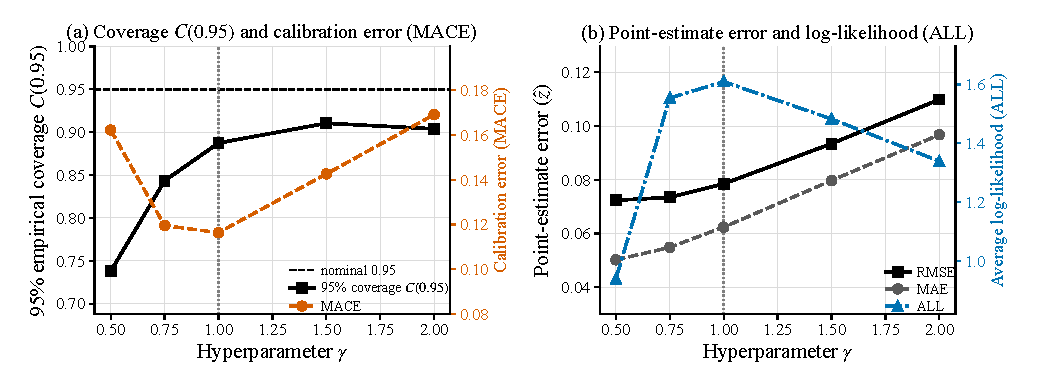
\includegraphics[width=0.98\textwidth]{figures_final/Fig_gamma_sensitivity.pdf}
\caption{Sensitivity of the performance metrics to the hyperparameter $\gamma$ on the validation dataset (2,400
observations, all stiffness factors): (a)~95\% empirical coverage $C(0.95)$ (left axis) and mean absolute calibration
error (MACE, right axis); (b)~root-mean-square error (RMSE) and mean absolute error (MAE) of the posterior mean
$\hat{\z}$ (left axis) and average log-likelihood (ALL, right axis). The vertical dotted line marks $\gamma=1$.}
\label{fig:gamma_sensitivity}
\end{figure}

\begin{figure}[H]
\centering
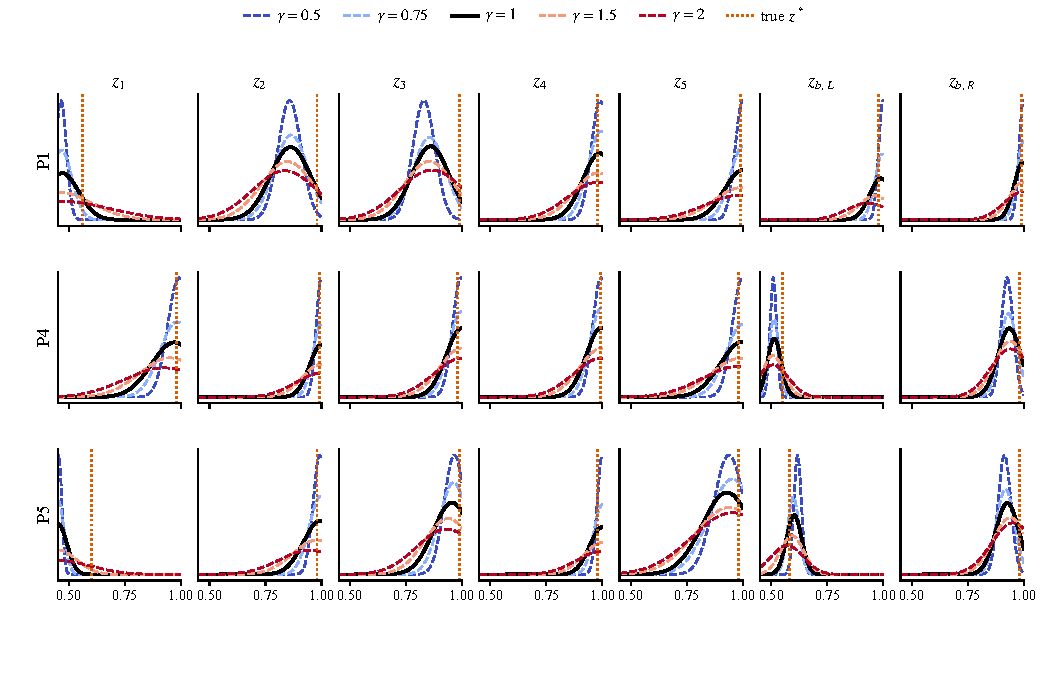
\includegraphics[width=0.98\textwidth]{figures_final/Fig_gamma_benchmarks_1D.pdf}
\caption{Effect of $\gamma\in\{0.5,0.75,1,1.5,2\}$ on the 1D marginal posteriors $q_\gamma(z_d|\m)$ of benchmark
scenarios P1, P4, and P5. Varying $\gamma$ scales the width of the marginal posteriors while keeping their mode aligned
with the true stiffness factor $z^*$ (vertical dotted line); near the upper bound $z=1$, wider truncated marginals
become more skewed toward lower values, shifting their mean downward.}
\label{fig:gamma_benchmarks_1D}
\end{figure}

\begin{action}
Section ``Sensitivity to $\gamma$ hyperparameter and model selection'' rewritten using the validation dataset only
\lines{xx--yy}, with Table~\tbd{x} (Table~\ref{tab:gamma_sensitivity}) and Figs.~\tbd{x--y}
(Figs.~\ref{fig:gamma_sensitivity} and~\ref{fig:gamma_benchmarks_1D}); unbiased test-set metrics reported in
Table~\tbd{x} (Table~\ref{tab:metricsB}, R1.3).
\end{action}

\end{document}
